%------------------------------------------------------------------------------
\section{Process noise modelling}
\label{sec:noise}
%------------------------------------------------------------------------------

\subsection{Overview}

Describing the motion of a satellite through the integration of the equations of motion, considering all acting perturbations, will typically lead to
deviations with respect to the true trajectory. The first step is to account for the uncertainties in the initial state via the covariance matrix, which results from the orbit
determination process, essentially the errors in the observations of the satellite.

However, an additional source of error is often neglected: force model errors are introduced during the propagation and are manifold, including
\begin{itemize}
 \item unmodeled perturbations,
 \item uncertainties in the coefficients of the geopotential,
 \item geopotential series truncation,
 \item stochastic nature of solar and geomagnetic activity,
 \item uncertainty in the ballistic coefficient,
 \item simplifications in modeling the optical properties, etc.
\end{itemize}
Most of the above mentioned effects may be described by a stochastic process. For many systems, such a process is well approximated by Gaussian white noise and is referred to 
as \gls{acr:snc}. A more sophisticated modeling, where process noise parameters are included in the state vector as solve-for parameters, is referred to as \gls{acr:dmc}. 
Both methods are described in detail by \citet{tapley2004}.

However, as \cite{nazarenko2010} points out, analysis for the geopotential model shows that the resulting errors are apparently non-Gaussian, a property generally denoted as
\textit{colored noise}. The difference between colored and white noise results from the uncertainties in the coefficients of the geopotential as well as a truncation of the
infinite series of the geopotential (\eq{eq:geopotential}), introducing considerably time-correlated errors.

In the following, the model to consider colored noise due to the geopotential shall be described, based on the book of \cite{nazarenko2010}. Being only available in Russian
language, some more details of the model from that book are provided here for convenience. A similar approach is also provided by \cite{wright1981} or \cite{wright2008}, however,
the cross-correlation of the state vector and the process noise, as introduced in \sect{sec:propagation-covariance-theory}, are not taken into consideration for the
computations therein.

The main difference between modeling colored noise as opposed to white noise, is that the cross-correlation matrix between the state vector and the process noise is non-zero,
\begin{equation}
 \gls{sym:expVal}\left[\Delta \gls{sym:state}\left(\gls{sym:t}_0\right) \gls{sym:inputVec}\left(\gls{sym:t}\right)^T\right] \neq 0,
\end{equation}
so that, from \eq{eq:full-cov-prop}, besides the solution of the double integral for \gls{sym:Quu}, an additional integral for \gls{sym:Qxu} needs to be computed.

\subsection{Modelling the errors of the geopotential}

The errors in the geopotential model contribute to the expected value, or the second moment of process noise, as present in the integral formulations for \gls{sym:Quu} and
\gls{sym:Qxu}, which were defined in \eq{eq:full-cov-prop}. They are given here again, for convenience:
\begin{align}
  \gls{sym:Quu}\left(\gls{sym:t}\right) &= \int_{\gls{sym:t}_0}^{\gls{sym:t}} \int_{\gls{sym:t}_0}^{\gls{sym:t}} \gls{sym:set}\left(\gls{sym:t},\gls{sym:xi}\right) \cdot
\gls{sym:inputMat}\left(\gls{sym:xi}\right) \cdot
\gls{sym:expVal}\left[\gls{sym:inputVec}\left(\gls{sym:xi}\right)\cdot \gls{sym:inputVec}\left(\gls{sym:eta}\right)^T\right]
\gls{sym:inputMat}\left(\gls{sym:eta}\right)^T \cdot
\gls{sym:set}\left(\gls{sym:t},\gls{sym:eta}\right)^T d\gls{sym:xi} d\gls{sym:eta} \label{eq:quu}\\
\gls{sym:Qxu}\left(\gls{sym:t}\right) &=
\gls{sym:set}\left(\gls{sym:t},\gls{sym:t}_0\right)\cdot\int_{\gls{sym:t}_0}^{\gls{sym:t}}\gls{sym:expVal}\left[\Delta\gls{sym:state}\left(\gls{sym:t}_0\right)
\cdot\gls{sym:inputVec}\left(\gls{sym:eta}\right)^T\right]\cdot\gls{sym:inputMat}\left(\gls{sym:eta}\right)\cdot
\gls{sym:set}\left(\gls{sym:t},\gls{sym:eta}\right) d\gls{sym:eta}
\end{align}
The process noise function is given in an orbit-centered reference frame as a $3\times 1$ vector:
\begin{equation}
 \gls{sym:inputVec}\left(\gls{sym:t}\right) = \left(\Delta \gls{sym:specForce}_{\gls{idx:radial}}, \Delta \gls{sym:specForce}_{\gls{idx:along}}, \Delta
\gls{sym:specForce}_{\gls{idx:normal}}\right)^T, \label{eq:force-model-errors}
\end{equation}
here, $\Delta \gls{sym:specForce}_{\gls{idx:radial}}$ is the error in the force model in radial, $\Delta \gls{sym:specForce}_{\gls{idx:along}}$ in along-track and $\Delta
\gls{sym:specForce}_{\gls{idx:normal}}$ in orbit normal direction, respectively. 

The following functions are introduced to simplify the formulas in the subsequent derivation:
\begin{align}
 \rhon{\gls{sym:geo_n}}\left(\gls{sym:r}\right)  &= \frac{\gls{sym:grav}}{\gls{sym:r}^2}\left(\frac{\re}{\gls{sym:r}}\right)^{\gls{sym:geo_n}}\\
 \fnk{\gls{sym:geo_n}}{\gls{sym:geo_m}} \left(\gls{sym:long}\right) &= \Delta\cnm{}{} \cos \left(\gls{sym:geo_m}\gls{sym:long}\right) + \Delta\snm{}{} \sin
\left(\gls{sym:geo_m}\gls{sym:long}\right) \\
 \gnk{\gls{sym:geo_n}}{\gls{sym:geo_m}} \left(\gls{sym:long}\right) &= \Delta\snm{}{} \cos \left(\gls{sym:geo_m}\gls{sym:long}\right) - 
\Delta\cnm{}{} \sin \left(\gls{sym:geo_m}\gls{sym:long}\right),
\end{align}
where $\Delta\cnm{}{}$ and $\Delta\snm{}{}$ are desribing the model errors introduced through both, truncation (\textit{error of omission}), which means that the geopotential is
considered up to a maximum degree of $\gls{sym:geo_n}_{max}$, as well as uncertainties in the estimation of the coefficients of the harmonic series (\textit{error of commission}):
\begin{align}
 \Delta\cnm{}{},\Delta\snm{}{} = \begin{cases}
                                  \left(\cnm{}{}-\hat{\gls{sym:geo_C}}_{\gls{sym:geo_n}\gls{sym:geo_m}}\right),
\left(\snm{}{}-\hat{\gls{sym:geo_S}}_{\gls{sym:geo_n}\gls{sym:geo_m}}\right) & \mbox{if } \gls{sym:geo_n}\leq\gls{sym:geo_n}_{max} \\
                                  \cnm{}{}, \snm{}{} & \mbox{if } \gls{sym:geo_n}>\gls{sym:geo_n}_{max}
                                 \end{cases} \label{eq:deltaCS}
\end{align}
here, $\hat{\gls{sym:geo_C}}_{\gls{sym:geo_n}\gls{sym:geo_m}}$ and $\hat{\gls{sym:geo_S}}_{\gls{sym:geo_n}\gls{sym:geo_m}}$ are the nominal values, or best estimates, of the
harmonic coefficients. For the \acrshort{acr:eigen}-GL04C the mean value and the standard deviations of the coefficients are shown in \fig{fig:eigen-gl04c} as a
function of the geopotential degree \gls{sym:geo_n}.
\begin{figure}[h!]
  \centering
  \begin{tikzpicture} 
  \begin{semilogyaxis}[
      %y tick label style={
      %  /pgf/number format/.cd,
      %      fixed,
      %      fixed zerofill,
      %      precision=1,
      %  /tikz/.cd
      % },
      x tick label style={
       /pgf/number format/.cd,
           fixed,
           fixed zerofill,
           precision=0,
       /tikz/.cd
      },
       width=0.7\textwidth,
       scaled x ticks = false,
       xlabel = {Geopotential degree},
       ylabel = Value,
       xmin=3,
       xmax=70,
       %clip=false,
       %xtick={0,1,2,3,4,5,6,7},
       grid=major,
       legend entries={Mean values of degree \gls{sym:geo_n}, Kaula's rule, Standard deviation of degree \gls{sym:geo_n}},
       %legend style={at={(1.2,0.5)}, anchor=west, draw=none},
       legend cell align = left
      ]
      
      \addplot[dark-red, mark=x] table {07-Tikz/data/coeff_eigen_gl04c.dat};
      \addplot[domain=3:70, samples=100] {1e-5/x^2};
      \addplot[ilr-blue, mark=o] table {07-Tikz/data/csig_eigen_gl04c.dat}; 
  \end{semilogyaxis}
 \end{tikzpicture}
  \caption{Mean value of the normalized spherical harmonic coefficients, as well as the normalized standard deviations as a function of the geopotential degree. Also
shown is
Kaula's approximation.\label{fig:eigen-gl04c}}
\end{figure}
The mean value for a certain degree \gls{sym:geo_n} is computed via a formulation given by \citet{kaula2000}:
\begin{equation}
 \gls{sym:mean}_{\gls{sym:geo_n}} = \sqrt{\frac{1}{2\gls{sym:geo_n}+1}\sum_{\gls{sym:geo_m}=0}^{\gls{sym:geo_n}} \left(\ncnm{}{}^2+\nsnm{}{}^2\right)}
\end{equation}
Kaula also provided an approximation to estimate the magnitude of the normalized coefficients, given the degree \gls{sym:geo_n}:
\begin{equation}
 \gls{sym:mean}_{\gls{sym:geo_n}} \approx \frac{\num{e-5}}{\gls{sym:geo_n}^2}. \label{eq:kaula}
\end{equation}
The standard deviation for the geopotential degree \gls{sym:geo_n} is computed according to \citet{nazarenko2010}:
\begin{equation}
 \gls{sym:stdev}_{\gls{sym:geo_n}}=\frac{1}{2\gls{sym:geo_n}+1}\sum_{\gls{sym:geo_m}+1}^{\gls{sym:geo_n}}\left(\gls{sym:stdev}\left(\ncnm{}{}\right)+
 \gls{sym:stdev}\left(\nsnm{}{}\right)\right).
\end{equation}


The force model errors, as required in \eq{eq:force-model-errors}, are obtained in two steps. The first step is to obtain the derivatives of the geopotential with respect to the
radius, the geocentric latitude and longitude, respectively (using only the perturbing part, see also \eq{eq:geopotential} and \eq{eq:deriv-geopotential}):
\begin{align}
 \Delta \gls{sym:specForce}_{\gls{idx:radial}} &= 
       \Delta \left(\frac{\partial \gls{sym:potential}}{\partial \gls{sym:r}}\right) = -\sum\limits_{\gls{sym:geo_n}=2}^{\infty} \rhon{\gls{sym:geo_n}}\left(\gls{sym:r}\right)
\left(\gls{sym:geo_n}+1\right) \sum\limits_{\gls{sym:geo_m}=0}^{\gls{sym:geo_n}} \fnk{\gls{sym:geo_n}}{\gls{sym:geo_m}} \left(\gls{sym:long}\right) \legphi{}{} \label{eq:dfr}\\
 \Delta \gls{sym:specForce}_{\gls{idx:lat}}  &= 
       \Delta \left(\frac{1}{\gls{sym:r}}\frac{\partial\gls{sym:potential}}{\partial\phigc}\right) = \sum\limits_{\gls{sym:geo_n}=2}^{\infty}
\rhon{\gls{sym:geo_n}}\left(\gls{sym:r}\right) \sum\limits_{\gls{sym:geo_m}=0}^{\gls{sym:geo_n}} \fnk{\gls{sym:geo_n}}{\gls{sym:geo_m}} \left(\gls{sym:long}\right)
\frac{\partial}{\partial \phigc} \legphi{}{} \label{eq:dfphi} \\
 \Delta \gls{sym:specForce}_{\gls{idx:lon}} &= \Delta \left(\frac{1}{\gls{sym:r}\cos\phigc}\frac{\partial\gls{sym:potential}}{\partial\gls{sym:long}}\right) =
    \sum\limits_{\gls{sym:geo_n}=2}^{\infty} \rhon{\gls{sym:geo_n}}\left(\gls{sym:r}\right) \sum\limits_{\gls{sym:geo_m}=0}^{\gls{sym:geo_n}} 
      \frac{\gls{sym:geo_m}}{\cos\phigc}\gnk{\gls{sym:geo_n}}{\gls{sym:geo_m}} \left(\gls{sym:long}\right)\legphi{}{} \label{eq:dflam}
\end{align}
Assuming that the mean (expected value) of \eq{eq:dfr} through \eq{eq:dflam} is zero, the variance in radius, geocentric latitude and longitude direction, respectively, can be
obtained as:
\begin{align}
 \gls{sym:stdev}_{\gls{idx:radial}}^2 \left(\gls{sym:r},\phigc,\gls{sym:long}\right) &= \gls{sym:expVal}\left[\Delta \gls{sym:specForce}_{\gls{idx:radial}}^2\right]
       = \gls{sym:expVal}\left[\sum\limits_{j=2}^{\infty}\sum\limits_{\gls{sym:geo_n}=2}^{\infty} \rhon{j}\rhon{\gls{sym:geo_n}}
       \left(j+1\right)\left(\gls{sym:geo_n}+1\right) \sum\limits_{i=0}^{j}\sum\limits_{\gls{sym:geo_m}=0}^{\gls{sym:geo_n}}
\fnk{j}{i}\fnk{\gls{sym:geo_n}}{\gls{sym:geo_m}} \gls{sym:legendre}_{j,i}\gls{sym:legendre}_{\gls{sym:geo_n},\gls{sym:geo_m}}\right] \label{eq:sigmaRad}\\
 \gls{sym:stdev}_{\gls{idx:lat}}^2 \left(\gls{sym:r},\phigc,\gls{sym:long}\right) &= \gls{sym:expVal}\left[\Delta \gls{sym:specForce}_{\gls{idx:lat}}^2\right]
 = \gls{sym:expVal}\left[\sum\limits_{j=2}^{\infty}\sum\limits_{\gls{sym:geo_n}=2}^{\infty} \rhon{j}\rhon{\gls{sym:geo_n}}
       \sum\limits_{i=0}^{j}\sum\limits_{\gls{sym:geo_m}=0}^{\gls{sym:geo_n}}
\fnk{j}{i}\fnk{\gls{sym:geo_n}}{\gls{sym:geo_m}} \frac{\partial\gls{sym:legendre}_{j,i}}{\partial
\phigc}\frac{\partial\gls{sym:legendre}_{\gls{sym:geo_n},\gls{sym:geo_m}}}{\partial \phigc}\right]
       \\
 \gls{sym:stdev}_{\gls{idx:lon}}^2 \left(\gls{sym:r},\phigc,\gls{sym:long}\right) &= \gls{sym:expVal}\left[\Delta \gls{sym:specForce}_{\gls{idx:lon}}^2\right]
       = \gls{sym:expVal}\left[\sum\limits_{j=2}^{\infty}\sum\limits_{\gls{sym:geo_n}=2}^{\infty} \rhon{j}\rhon{\gls{sym:geo_n}}
       \sum\limits_{i=0}^{j}\sum\limits_{\gls{sym:geo_m}=0}^{\gls{sym:geo_n}} \frac{i\gls{sym:geo_m}}{\cos^2\phigc}\gnk{j}{i}\gnk{\gls{sym:geo_n}}{\gls{sym:geo_m}}
\gls{sym:legendre}_{j,i}\gls{sym:legendre}_{\gls{sym:geo_n},\gls{sym:geo_m}}\right] \label{eq:sigmaLam}
\end{align}
The expected value for a univariate continuous random variable can be computed as:
\begin{equation}
 \gls{sym:expVal}\left[\gls{sym:Z}\right] = \int_{-\infty}^{\infty} \gls{sym:zg} \gls{sym:probDens}\left(\gls{sym:zg}\right) d\gls{sym:zg}.
\end{equation}
For a unity sphere, points can be distributed uniformly so that for the surface area of $\gls{sym:area}=4\gls{sym:pi}$ the probability density function is given
as:
\begin{equation}
 \gls{sym:probDens}\left(\gls{sym:Z}\right) = \gls{sym:probDens}\left(\gls{sym:r}, \phigc, \gls{sym:long}\right) = \frac{1}{4\gls{sym:pi}}.
\end{equation}
The expected value in spherical coordinates for a given radial distance \gls{sym:r} is then
\begin{equation}
 \gls{sym:expVal}\left[\gls{sym:Z}\left(\gls{sym:r},\phigc,\gls{sym:long}\right)\right] =
\frac{1}{4\gls{sym:pi}}\int_{-\gls{sym:pi}/2}^{\gls{sym:pi}/2}\left(\int_{0}^{2\gls{sym:pi}}
\gls{sym:Z}\left(\gls{sym:r},\phigc,\gls{sym:long}\right)d\gls{sym:long}\right)\cos\phigc d\phigc. \label{eq:expval-z}
\end{equation}

\subsubsection{Integral evaluation for longitude functions}

In \eq{eq:expval-z} the inner integral is with respect to the longitude, which results in evaluating
\begin{align}
 \int_{0}^{2\gls{sym:pi}} \fnk{\gls{sym:geo_n}}{\gls{sym:geo_m}}\left(\gls{sym:long}\right) \fnk{j}{i}\left(\gls{sym:long}\right) d\gls{sym:long} &=
  \frac{1}{2}\Delta\cnm{}{}\Delta\cij{}{}
\int_{0}^{2\gls{sym:pi}}\left(\cos\left(\gls{sym:geo_m}-i\right)\gls{sym:long}+\cos\left(\gls{sym:geo_m}+i\right)\gls{sym:long}\right) d\gls{sym:long} + \notag \\
 &+ \frac{1}{2}\Delta\snm{}{}\Delta\sij{}{}
\int_{0}^{2\gls{sym:pi}}\left(\cos\left(\gls{sym:geo_m}-i\right)\gls{sym:long}-\cos\left(\gls{sym:geo_m}+i\right)\gls{sym:long}\right) d\gls{sym:long} +  \\
 &+ \frac{1}{2}\left(\Delta\cnm{}{}\Delta\sij{}{}+\Delta\snm{}{}\Delta\cij{}{}\right)
\int_{0}^{2\gls{sym:pi}}\left(\sin\left(\gls{sym:geo_m}-i\right)\gls{sym:long}+\sin\left(\gls{sym:geo_m}+i\right)\gls{sym:long}\right) d\gls{sym:long}. \notag
\end{align}
The above integrals are all zero for $\gls{sym:geo_m} \neq i$. If $\gls{sym:geo_m}=i \neq 0$, only the cosine functions with arguments
$\left(\gls{sym:geo_m}-i\right)\gls{sym:long}$ provide non-zero contributions, while for $\gls{sym:geo_m}=i=0$ only zonal harmonics remain (as
$\Delta\gls{sym:geo_S}_{\gls{sym:geo_n},0}= \Delta\gls{sym:geo_S}_{j,0} =0$). Therefore, the result of the integral evaluation is
\begin{equation}
 \int_{0}^{2\gls{sym:pi}} \fnk{\gls{sym:geo_n}}{\gls{sym:geo_m}}\left(\gls{sym:long}\right) \fnk{j}{i}\left(\gls{sym:long}\right) d\gls{sym:long} 
 = \begin{cases}
   0 & \mbox{if } \gls{sym:geo_m} \neq i, \\
   \frac{2\gls{sym:pi}}{\gls{sym:deltam}}\left(\Delta\cnm{}{}\Delta\cij{}{}+\Delta\snm{}{}\Delta\sij{}{}\right) & \mbox{if } \gls{sym:geo_m} = i,
   \end{cases} \label{eq:integral-ff}
\end{equation}
where \gls{sym:deltam} is according to the definition in \eq{eq:normalization}. The same result is obtained for the derivatives functions:
\begin{equation}
 \int_{0}^{2\gls{sym:pi}} \gnk{\gls{sym:geo_n}}{\gls{sym:geo_m}}\left(\gls{sym:long}\right) \gnk{j}{i}\left(\gls{sym:long}\right) d\gls{sym:long} 
 = \begin{cases}
   0 & \mbox{if } \gls{sym:geo_m} \neq i, \\
   \frac{2\gls{sym:pi}}{\gls{sym:deltam}}\left(\Delta\cnm{}{}\Delta\cij{}{}+\Delta\snm{}{}\Delta\sij{}{}\right) & \mbox{if } \gls{sym:geo_m} = i,
   \end{cases}
\end{equation}

\subsubsection{Integral evaluation for Legendre functions}

The outer integral in \eq{eq:expval-z} results in evaluating three different integrals for the combined Legendre functions in \eq{eq:sigmaRad} through \eq{eq:sigmaLam}.
Using the known orthogonality relations for the Legendre polynomials (e.g. \citet{abramowitz1964}), the first integral is easily obtained as:
\begin{align}
 \int_{-\gls{sym:pi}/2}^{\gls{sym:pi}/2} \gls{sym:legendre}_{\gls{sym:geo_n},\gls{sym:geo_m}}\left(\sin\phigc\right)
\gls{sym:legendre}_{j,i}\left(\sin\phigc\right) \cos\phigc d\phigc &= \int_{-1}^{1}
\gls{sym:legendre}_{\gls{sym:geo_n},\gls{sym:geo_m}}\left(\sin\phigc\right)
\gls{sym:legendre}_{j,i}\left(\sin\phigc\right) d\left(\sin\phigc\right) \notag \\
 &= \begin{cases}
     0 & \mbox{if } \gls{sym:geo_n} \neq j, \\
     \frac{2\left(\gls{sym:geo_n}+\gls{sym:geo_m}\right)!}{\left(2\gls{sym:geo_n}+1\right)\left(\gls{sym:geo_n}-\gls{sym:geo_m}\right)!} & \mbox{if } \gls{sym:geo_n} = j.
    \end{cases} \label{eq:legendre-orth-1}
\end{align}
The other two integrals involve a lengthy process to obtain the final result, which is given in full detail in the Appendix of \citet{nazarenko2010}:
\begin{align}
 \int_{-1}^{1} \gls{sym:legendre}_{\gls{sym:geo_n},\gls{sym:geo_m}}\left(\sin\phigc\right)
\gls{sym:legendre}_{j,i}\left(\sin\phigc\right) \frac{1}{\cos^2\phigc} d\left(\sin\phigc\right) &= 
    \begin{cases}
      0 & \mbox{if } \gls{sym:geo_n} \neq j, \\
     \frac{\left(\gls{sym:geo_n}+\gls{sym:geo_m}\right)!}{\gls{sym:geo_m}\left(\gls{sym:geo_n}-\gls{sym:geo_m}\right)!} & \mbox{if } \gls{sym:geo_n} = j.
    \end{cases}     \\
 \int_{-1}^{1} \frac{\partial \gls{sym:legendre}_{\gls{sym:geo_n},\gls{sym:geo_m}}\left(\sin\phigc\right)}{\partial \phigc}
\frac{\partial \gls{sym:legendre}_{j,i}\left(\sin\phigc\right)}{\partial \phigc} d\left(\sin\phigc\right) &= 
    \begin{cases}
      0 & \mbox{if } \gls{sym:geo_n} \neq j, \\    
\frac{\left(\gls{sym:geo_n}+\gls{sym:geo_m}\right)!}{\left(\gls{sym:geo_n}-\gls{sym:geo_m}\right)!}\left(\frac{2\gls{sym:geo_n}\left(\gls{sym:geo_n}+1\right)}{2
\gls{sym:geo_n}+1}-\gls{sym:geo_m} \right) & \mbox{if } \gls{sym:geo_n} = j.
    \end{cases} 
\end{align}

\subsubsection{Force model variances in spherical coordinates}

With the integrals being evaluated, the result for the variances, as introduced in \eq{eq:sigmaRad} through \eq{eq:sigmaLam}, can finally be written for the spherical
coordinate system. For the radial variance, by using the results from \eq{eq:integral-ff} and \eq{eq:legendre-orth-1} one obtains:
\begin{align}
 \gls{sym:stdev}_{\gls{idx:radial}}^2\left(\gls{sym:r}\right) = \frac{1}{4\gls{sym:pi}} \sum_{\gls{sym:geo_n}=2}^{\infty}
 \rhon{\gls{sym:geo_n}}^2\left(\gls{sym:geo_n}+1\right)^2\sum_{\gls{sym:geo_m}=0}^{\gls{sym:geo_n}}
\frac{2\left(\gls{sym:geo_n}+\gls{sym:geo_m}\right)!}{\gls{sym:deltam}\left(2\gls{sym:geo_n}+1\right)\left(\gls{sym:geo_n}-\gls{sym:geo_m}\right)!}2\gls{sym:pi}
\left(\Delta\cnm{}{}^2+\Delta\snm{}{}^2\right),
\end{align}
which simplifies as soon as normalized coefficients are considered using \eq{eq:normalization}:
\begin{align}
 \gls{sym:stdev}_{\gls{idx:radial}}^2\left(\gls{sym:r}\right) = \left(\frac{\gls{sym:grav}}{\gls{sym:r}^2}\right)^2 \sum_{\gls{sym:geo_n}=2}^{\infty}
 \left(\frac{\re}{\gls{sym:r}}\right)^{2\gls{sym:geo_n}}\left(\gls{sym:geo_n}+1\right)^2\sum_{\gls{sym:geo_m}=0}^{\gls{sym:geo_n}}
\left(\Delta\ncnm{}{}^2+\Delta\nsnm{}{}^2\right). \label{eq:stdev-rad}
\end{align}
For the variances in longitude and latitude direction, the derivation is analogously:
\begin{align}
 \gls{sym:stdev}_{\gls{idx:lat}}^2\left(\gls{sym:r}\right) &= \frac{1}{2}\left(\frac{\gls{sym:grav}}{\gls{sym:r}^2}\right)^2 \sum_{\gls{sym:geo_n}=2}^{\infty}
 \left(\frac{\re}{\gls{sym:r}}\right)^{2\gls{sym:geo_n}}\left(2\gls{sym:geo_n}+1\right)\sum_{\gls{sym:geo_m}=0}^{\gls{sym:geo_n}}
\left(\frac{2\gls{sym:geo_n}\left(\gls{sym:geo_n}+1\right)}{2\gls{sym:geo_n}+1}-\gls{sym:geo_m}\right)\left(\Delta\ncnm{}{}^2+\Delta\nsnm{}{}^2\right). \\
 \gls{sym:stdev}_{\gls{idx:lon}}^2\left(\gls{sym:r}\right) &= \frac{1}{2}\left(\frac{\gls{sym:grav}}{\gls{sym:r}^2}\right)^2 \sum_{\gls{sym:geo_n}=2}^{\infty}
 \left(\frac{\re}{\gls{sym:r}}\right)^{2\gls{sym:geo_n}}\left(2\gls{sym:geo_n}+1\right)\sum_{\gls{sym:geo_m}=0}^{\gls{sym:geo_n}} \gls{sym:geo_m}
\left(\Delta\ncnm{}{}^2+\Delta\nsnm{}{}^2\right).\label{eq:stdev-lon}
\end{align}
The individual variances are a function of the geocentric radius. For a selected geopotential model, the harmonic coefficients and their standard deviations are required
for the evaluation. According to the definition of the quantities $\Delta\ncnm{}{}$ and $\Delta\nsnm{}{}$ in \eq{eq:deltaCS}, the standard
deviations of the harmonic coefficients are summed up to the maximum degree of the geopotential considered in the propagation
($\gls{sym:geo_n}\leq\gls{sym:geo_n}_{max}$), while the harmonic coefficients are used for $\gls{sym:geo_n} > \gls{sym:geo_n}_{max}$. As \citet{nazarenko2010} points
out, the computation of the series in \eq{eq:stdev-rad} through \eq{eq:stdev-lon} can be carried out in two ways:
\begin{itemize}
 \item For $\gls{sym:geo_n}_{max}$ being small, the series will be truncated early, so that the error due to omission will be dominated by larger terms, with the
influence of terms of increasing order quickly declining. This means that the series with respect to the geopotential degree would be evaluated up to $\gls{sym:geo_n}
\approx 30\ldots40$.
 \item For the geopotential being considered to a high degree for high precise computations, the truncation sets in late and the amount of terms that are non-negligible
will be higher than in the case above. In order to reduce computational burden, \citet{nazarenko2010} recommends to use Kaula's rule \citep{kaula2000} for an efficient
evaluation (see \eq{eq:kaula}).
\end{itemize}
The second moment of process noise, which is required to evaluate \eq{eq:quu}, can be written in spherical coordinates as
\begin{equation}
 \gls{sym:expVal}\left[\gls{sym:inputVec}\gls{sym:inputVec}^T\right] = \gls{sym:expVal}\left[\begin{matrix}
                                                       \Delta \gls{sym:specForce}_{\gls{idx:radial}}^2 & \Delta \gls{sym:specForce}_{\gls{idx:radial}} \Delta
\gls{sym:specForce}_{\gls{idx:lat}} & \Delta \gls{sym:specForce}_{\gls{idx:radial}} \Delta \gls{sym:specForce}_{\gls{idx:lon}} \\
\Delta \gls{sym:specForce}_{\gls{idx:lat}} \Delta \gls{sym:specForce}_{\gls{idx:radial}} & \Delta \gls{sym:specForce}_{\gls{idx:lat}}^2 & \Delta
\gls{sym:specForce}_{\gls{idx:lat}} \Delta \gls{sym:specForce}_{\gls{idx:lon}} \\
\Delta \gls{sym:specForce}_{\gls{idx:lon}} \Delta \gls{sym:specForce}_{\gls{idx:radial}} & \Delta \gls{sym:specForce}_{\gls{idx:lon}} \Delta
\gls{sym:specForce}_{\gls{idx:lat}} & \Delta \gls{sym:specForce}_{\gls{idx:lon}}^2
\end{matrix} 
\right]= \left(\begin{matrix}
                 \gls{sym:stdev}_{\gls{idx:radial}}^2 & 0 & 0 \\
                 0 & \gls{sym:stdev}_{\gls{idx:lat}}^2 & 0 \\
                 0 & 0 & \gls{sym:stdev}_{\gls{idx:lon}}^2
                \end{matrix}
\right),
\end{equation}
where the non-diagonal terms are derived in a similar manner. As pointed out by \citet{nazarenko2010}, they are all zero.

TBC.

\begin{figure}[h!]
  \centering
  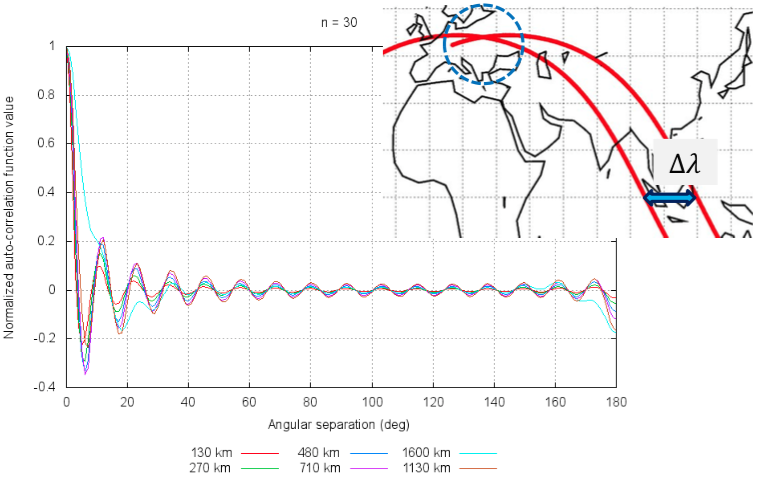
\includegraphics[width=\textwidth]{auto-correlation.png}
  \caption{Normalized auto-correlation function for the EIGEN-GL04C geopotential as a function of angular separation and the orbit altitude being the parameter. \label{fig:auto-correlation}} 
\end{figure}
\todo[Replace figure]{Replace \fig{fig:auto-correlation} using Tikz}

\subsection{Exemplary results}

\begin{figure}[h!]
  \centering
  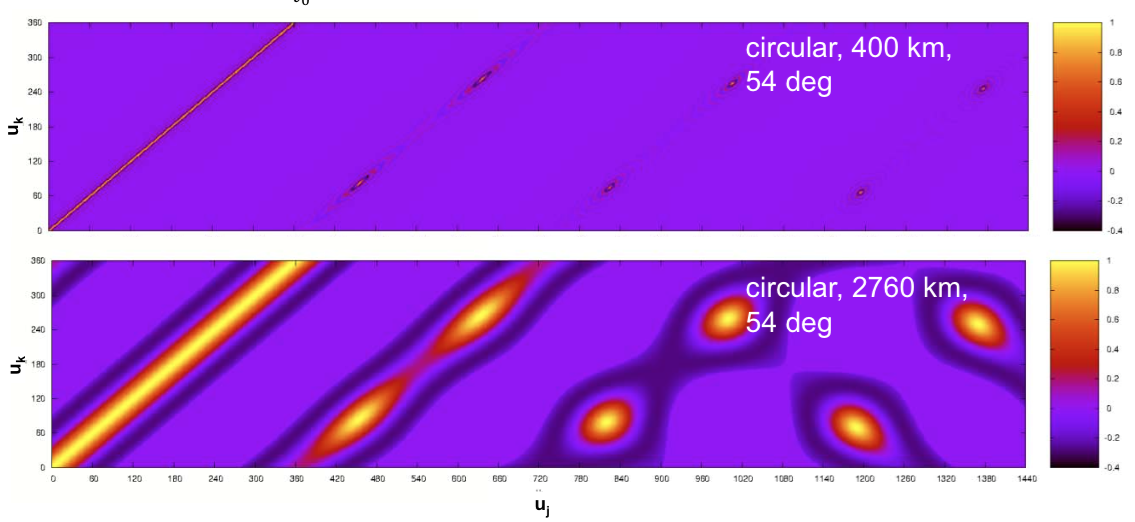
\includegraphics[width=\textwidth]{correlation-leo.png}
  \caption{Normalized auto-correlation function for two \gls{acr:leo} orbits, showing also the correlation of the current with subsequent orbits.\label{fig:correlation-leo}}
\end{figure}
\todo[Replace figure]{Replace \fig{fig:correlation-leo} using Tikz}

\begin{figure}[h!]
  \centering
  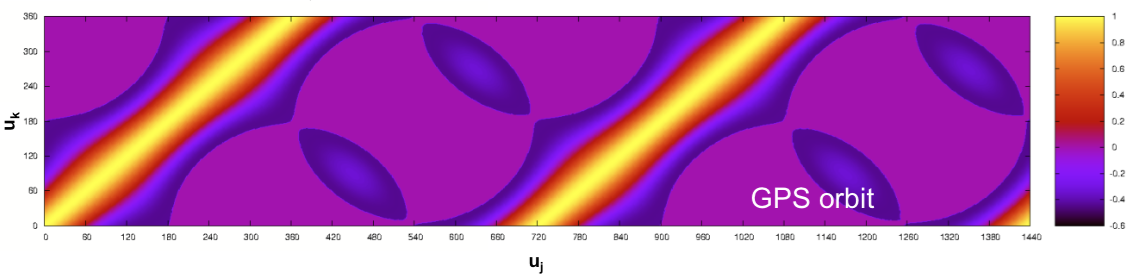
\includegraphics[width=\textwidth]{correlation-gps.png}
  \caption{Normalized auto-correlation function for \gls{acr:gps} orbits, showing also the correlation of the current with subsequent orbits. A typical picture for \SI{12}{\hour} resonance orbits.\label{fig:correlation-gps}}
\end{figure}
\todo[Replace figure]{Replace \fig{fig:correlation-gps} using Tikz}

\begin{figure}[h!]
  \centering
  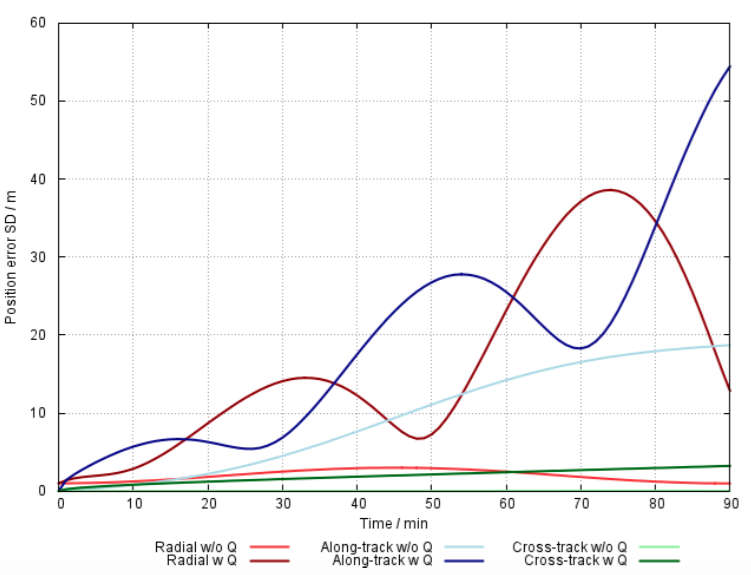
\includegraphics[width=\textwidth]{noise-results-matQ.png}
  \caption{Force model error contributions using a 30 $\times$ 30 geopotential, for an orbit at \SI{300}{\kilo\metre} and an inclination of \ang{50;;}.  \label{fig:noise-contributions}}
\end{figure}
\todo[Replace figure]{Replace \fig{fig:noise-contributions} using Tikz}


